\documentclass{beamer}

\usepackage{beamerthemeCVC}

\usepackage{graphicx}

\setbeamertemplate{caption}[numbered]

\usepackage{xmpmulti}

%% PRESENTATION CONFIGURATION PARAMETERS %%%%%%%%%%%%%%%%%%%%%%%%%%%%%%%%%%%%%%%
%  \titlebackgroundfile{images/template_title}
%  \framebackgroundfile{images/template_frame_v05}


%\definecolor{vermell}{HTML}{8C2423}
\definecolor{vermell}{HTML}{000066}
\definecolor{gris}{HTML}{4C4C4C}

% http://latexcolor.com/
\definecolor{anti-flashwhite}{rgb}{0.95, 0.95, 0.96}
\definecolor{palesilver}{rgb}{0.79, 0.75, 0.73}

 
%Font 
% \usefonttheme{professionalfonts}
% \usepackage[utf8]{inputenc}
\usefonttheme{default}

\usefonttheme[onlymath]{serif}
% http://tex.stackexchange.com/questions/34265/how-to-get-beamer-math-to-look-like-article-math



% http://tex.stackexchange.com/questions/183052/what-are-all-the-possible-first-arguments-to-setbeamerfont/183053#183053



\setbeamercolor{title in head/foot}{fg=vermell}


\setbeamercolor{author in head/foot}{fg=palesilver}
% 
\setbeamercolor{framenumber in head/foot}{fg=vermell}



\setbeamercolor{section in head/foot}{fg=vermell}
\setbeamercolor{normal text}{fg=gris}
%\setbeamercolor{frametitle}{fg=vermell}
\setbeamercolor{frametitle}{fg=blue!20!black}

\setbeamerfont{block title}{size={}}
\setbeamerfont{author}{size=\footnotesize}
\setbeamerfont{date}{size=\footnotesize}

\setbeamerfont{footline}{size=\fontsize{3}{11}\selectfont}


\setbeamertemplate{itemize item}[circle]
\setbeamertemplate{itemize subitem}[circle]
\setbeamertemplate{itemize subsubitem}[circle]
\setbeamertemplate{itemize subsubsubitem}[circle]
\setbeamercolor{itemize item}{fg=vermell}
\setbeamercolor{itemize subitem}{fg=vermell}
\setbeamercolor{itemize subsubitem}{fg=vermell}
\setbeamercolor{itemize subsubsubitem}{fg=vermell}
\setbeamercolor{enumerate item}{fg=vermell}
\setbeamercolor{enumerate subitem}{fg=vermell}
\setbeamercolor{enumerate subsubitem}{fg=vermell}
\setbeamercolor{enumerate subsubsubitem}{fg=vermell}
\setbeamercolor{alerted text}{fg=vermell}
\setbeamerfont{alerted text}{series=\bfseries}
% This command makes that acrobat reader doesn't changes the colors of the slide
% when there are figures with transparencies.
\pdfpageattr {/Group << /S /Transparency /I true /CS /DeviceRGB>>}



%\setbeamerfont{bibliography entry author}{series=\bfseries}
% \setbeamerfont{bibliography entry title}{series=\bfseries}
% \setbeamerfont{bibliography item}{series=\bfseries}

\setbeamerfont{bibliography item}{size=\scriptsize}
\setbeamerfont{bibliography entry author}{size=\scriptsize}
\setbeamerfont{bibliography entry title}{size=\scriptsize}
\setbeamerfont{bibliography entry location}{size=\scriptsize}
\setbeamerfont{bibliography entry note}{size=\scriptsize}

% \usepackage{hyperref}
% \hypersetup{colorlinks=true, linkcolor=blue}
% \renewcommand*{\bibfont}{\scriptsize}

\graphicspath{{images/}}





%%%%%%%%%%%%%%%%%%%%%%%%%%%%%%%%%%%%%%%%%%%%%%%%%%%%%%%%%%%%%%%%%%%%%%%%%%%%%%%%

%      + Short title.               + Title which appears in the cover.
%      v                            v
%\title[Beamer presentation example]{Nonlinear Dynamics Approach to Human Activity Recognition Using Inertial Sensors}
\vspace{5mm}
\title[Automatic Indentification of Movement Variability]
{Automatic Indentification of \\ Movement Variability}
%       + Short author names which appear in the slides.
%       v
\author[Miguel Xochicale]
{   % Author names which appear in the cover page.
    %Perez-Xochicale Miguel Angel\inst{1}
    Miguel Xochicale
}
%          + Short affiliation which appears in the slides.
%          v
\institute[CVC-IIIA]
{   % Affiliation information which appears in the cover page.

      \vspace{5mm}
    \begin{tabular}{c}
    %\inst{1}Internal Research Conference 
    \end{tabular}
}
%     + Short acronym of the conference or date of the presentation.
%     v
\date[DEMO-2013]
{   % Conference name which appears in the cover page.
     \today
}





\begin{document}
% Creates the cover page.
\frame{\titlepage}



% 
% 
% %+++++++++++++++++++++++++++++++++++++++++++++++++++
% %+++++++++++++++++++++++++++++++++++++++++++++++++++
% \section{Literature Review}


%%%%%%%%%%%%%%%%%%
%%%%%%%%%%%%%%%%%%
%SECTION00



 
% %+++++++++++++++++++++++++++++++++++++++++++++++++++
\begin{frame}
  \frametitle{Mexican Tournament of Robotics 2013}
% 
% 
  \begin{figure}
 \includegraphics[width=1\textwidth]{hri_tmr2013_00}
\centering 
\caption{Human-Robot Interaction Dance Demo}
 \end{figure}
% 
% 
 \end{frame}






%+++++++++++++++++++++++++++++++++++++++++++++++++++
%+++++++++++++++++++++++++++++++++++++++++++++++++++
\section{Research Questions}

%+++++++++++++++++++++++++++++++++++++++++++++++++++
\begin{frame}
	\frametitle{Research Questions}

    \begin{itemize}

    
     \item Can we automatically identify the variability of: \\
      \begin{description}
       \item[(a)] simple human activities (gestures) and
       \item[(b)] complex human activities (dance)?
      \end{description}

      \item 
      Can we use the identification of variability as a
      index of skilled performance?
      
%      \item How can we model the variability of simple human activities ?
    
%     \item How can we apply Takens's Theorem and Principal Component Analysis
% 	  to characterise the variability of Human Activities?
     \end{itemize}
    
%     Can we model the variability of simple human activities ?

\end{frame}
%---------------------------------------------------







%+++++++++++++++++++++++++++++++++++++++++++++++++++
\begin{frame}
\frametitle{Activity Recognition Chain for Inertial Sensors}
\vspace{-0.7cm}


\begin{figure}[!htb]
\centering    
\includegraphics[width=0.85\textwidth]{banos2014_ARC_3}
\caption[PA]{Window Size impact in ARC
 \textcolor{red}{\textbf{ \cite{Banos2014} }}.
}  
\label{fig:sn}
\end{figure}



\end{frame}
%---------------------------------------------------






%+++++++++++++++++++++++++++++++++++++++++++++++++++
\begin{frame}
\frametitle{Activity Recognition Chain  from \\ wearable sensors}
\vspace{-0.7cm}


\begin{figure}[!htb]
\centering    
\includegraphics[width=1\textwidth]{ARC02}
\caption[PA]{ARC to recognise activities from wearable sensors.
 \textcolor{red}{\textbf{ \cite{Bulling2014} }}.
}  
\label{fig:sn}
\end{figure}



\end{frame}
%---------------------------------------------------







%+++++++++++++++++++++++++++++++++++++++++++++++++++
\begin{frame}
\frametitle{}
\vspace{-2mm}


\begin{figure}[!htb]
\centering    
\includegraphics[width=1\textwidth]{feature_extraction_v01}
\caption[PA]{Techniques applied to accelerometer sensor signals for feature extraction 
\textcolor{red}{\textbf{ \cite{Figo2010,Liao2015,Gupta2014,Fish2012,Zhang2011} }}.
}  
\label{fig:sn}
\end{figure}



\end{frame}
%---------------------------------------------------





%+++++++++++++++++++++++++++++++++++++++++++++++++++
\begin{frame}
\frametitle{Time-delay embedding}
\vspace{-0.7cm}


\begin{figure}[!htb]
\centering    
\includegraphics[width=1\textwidth]{frank_2012}
\caption[PA]{Time-delay embedding for walking (left), running (middle), and cycling (right) $m=3$, $\tau=4$ . 
 \textcolor{red}{\textbf{ \cite{Frank2010,Frank2012} }}.
}  
\label{fig:sn}
\end{figure}



\end{frame}
%---------------------------------------------------





%+++++++++++++++++++++++++++++++++++++++++++++++++++
\begin{frame}
\frametitle{Time-delay embedding}
\vspace{-0.7cm}


\begin{figure}[!htb]
\centering    
\includegraphics[width=0.6\textwidth]{sama_2013}
\caption[PA]{Time delay embeddings for gait patterns of two persons ($m=20$ for $\tau=1$, $\tau=4$ and $\tau=9$, respectively). 
 \textcolor{red}{\textbf{ \cite{Sama2013} }}.
}  
\label{fig:sn}
\end{figure}



\end{frame}
%---------------------------------------------------








\section{Stochastic Model}



%+++++++++++++++++++++++++++++++++++++++++++++++++++
\begin{frame}
\frametitle{Intrinsic Structure Signal}
\vspace{-0.7cm}

Additive noise is created to introduce variance in the amplitude.
\begin{equation}
 S_i = S_i^3 + \mathcal{N}( 0 , \sigma_a ^2), \quad  i = 1,2,3.
\end{equation}
Where $S$ is a regular sinusoid signal \textcolor{red}{\textbf{ \cite{Hammerla2011} }}.

*Low levels of additive noise correspond to precise movements.

\end{frame}
%---------------------------------------------------


%+++++++++++++++++++++++++++++++++++++++++++++++++++
\begin{frame}
\frametitle{Intrinsic Structure Signal}
\vspace{-0.7cm}

Structural noise is created to introduce variance in frequency , amplitude and local biases.

\begin{figure}[!htb]
\centering   
\includegraphics[width=0.5\textwidth]{hammerla2011_algorithm2}
\caption[PA]{
Structural Noise Algorithm \textcolor{red}{\textbf{ \cite{Hammerla2011} }}.
}  
\label{fig:asn}
\end{figure}
Where $S$ has a base frequency $v_0$, and $S^s$ is the distorted signal.

*Low levels of structural noise correspon to a well chosen strategy.


\end{frame}
%---------------------------------------------------





%+++++++++++++++++++++++++++++++++++++++++++++++++++
\begin{frame}
\frametitle{Structural Noise}
\vspace{-0.7cm}


\begin{figure}[!htb]
\centering    
\includegraphics[width=0.8\textwidth]{hammerla2011_structuralnoise}
\caption[PA]{
Three artificial signals that show the impact of additive noise and structural 
noise on sinusoid signals \textcolor{red}{\textbf{ \cite{Hammerla2011} }}.
%  \textbf{ \cite{Hammerla2011} }
}  
\label{fig:sn}
\end{figure}

 
 % Low levels of additive noise correspond to precise movements
% while low levels of structural noise correspon to a well chosen strategy.

Additive noise -- precision of movements \\
Structural noise -- strategy for motion


\end{frame}
%---------------------------------------------------




%+++++++++++++++++++++++++++++++++++++++++++++++++++
\begin{frame}
\frametitle{Additive Noise and Structural Noise}
\vspace{-0.7cm}

Artificial signals are modeled using:
\begin{equation}
 S(n) = A sin (2\pi f_o  n T_s  )  + \textbf{N}n
\end{equation} 

where $\textbf{A}$, $\textbf{F}$ and $\textbf{N}$ are normalised random vectors,
$n$ is the sample number and $T_s$ is the sampling period.

\vspace{5mm}
A normalised random vector $\textbf{X} = [ \textbf{X}_1, \textbf{X}_2, ..., \textbf{X}_n  ]$ is expressed as 
 $\textbf{X} \sim \mathcal{N}( \mu_X , \sigma_X ^2) $ with mean $\mu_X$ and variance $\sigma_X ^2$ 

% 
% \begin{equation}
%  S(n) = b_0 + a_0 sin (2\pi f_0 n T_s + \phi ) 
% \end{equation} 
% where $a_0$ is the amplitude, $f_0$ is the fundamental frequency,



\end{frame}
%---------------------------------------------------





%+++++++++++++++++++++++++++++++++++++++++++++++++++
\begin{frame}
\frametitle{Additive Noise and Structural Noise}
\vspace{-0.7cm}

% \begin{figure}
% \centering 
% \includegraphics[scale=0.12]{impactofnoise01} 
% \end{figure}

\begin{figure}[!htb]
\centering    
\includegraphics[width=1.0\textwidth]{impactofnoise01}
\caption[PA]{A, B, C and D plots present the variability of additive noise 
($\sigma_a ^2$) and structural noise ($\sigma_s ^2$ ) on sinusoid signals with window lenght $w_s=500$
\textcolor{red}{\textbf{[Hammerla 2011]}}.}
\label{fig:sn}
\end{figure}



\end{frame}
%---------------------------------------------------


%+++++++++++++++++++++++++++++++++++++++++++++++++++
\begin{frame}
\frametitle{Variation per cycle}
\vspace{5mm}

\begin{figure}[!htb]
\centering    
\includegraphics[width=1.0\textwidth]{variabilitydrawing00}
\caption[PA]{Variation of the Standard deviation for frenquency and amplitude values per cycle}
\label{}
\end{figure}



\end{frame}
%---------------------------------------------------



\section{Sensor Validation}
 
 
 
%+++++++++++++++++++++++++++++++++++++++++++++++++++
\begin{frame}
\frametitle{Gestures}
\vspace{-7mm}

\begin{figure}[!htb]
\centering    
\includegraphics[width=0.5\textwidth]{gestures_plotz2016_automatic_synchronization_of_wearable_sensors_and_video_cameras}
\caption[PA]{Vertical, horizontal, diagonal, circular and wave-like  \textcolor{red}{\textbf{ \cite{Plotz2012} }}.}
\label{}
\end{figure}




% Thomas Plotz et al ``Automatic Synchronization of Wearable Sensors and Video-Cameras for Ground Thuth Annotation --
% A Practical Approach. ISWC 2012
\end{frame}
%---------------------------------------------------
 
 

 
 
 
 
%+++++++++++++++++++++++++++++++++++++++++++++++++++
\begin{frame}
\frametitle{plotacc imu0 24022016-124306.csv}
\vspace{-7mm}

\begin{figure}[!htb]
\centering    
\includegraphics[width=1.0\textwidth]{plotacc_imu0_24022016-124306}
\caption[PA]{ACC imu0}
\label{}
\end{figure}

\end{frame}
%---------------------------------------------------
 


% +++++++++++++++++++++++++++++++++++++++++++++++++++
\begin{frame}
\frametitle{plotacc imu1 24022016-124306.csv}
\vspace{-7mm}

\begin{figure}[!htb]
\centering    
\includegraphics[width=1.0\textwidth]{plotacc_imu1_24022016-124306}
\caption[PA]{ACC imu1}
\label{}
\end{figure}

\end{frame}
%---------------------------------------------------
 
 
 


% +++++++++++++++++++++++++++++++++++++++++++++++++++
\begin{frame}
\frametitle{plotaccRAW Shimmer24022016-1242}
\vspace{-7mm}

\begin{figure}[!htb]
\centering    
\includegraphics[width=1.0\textwidth]{plotaccRAW_ShimmerData24022016-1242}
\caption[PA]{ACC Shimmer}
\label{}
\end{figure}

\end{frame}
%---------------------------------------------------




% +++++++++++++++++++++++++++++++++++++++++++++++++++
\begin{frame}
\frametitle{ imu0 vs imu1 }
\vspace{-7mm}

\begin{figure}[!htb]
\centering    
\includegraphics[width=1.0\textwidth]{plotacc_imu0_vs_imu124022016-124306}
\caption[PA]{comparison}
\label{}
\end{figure}

\end{frame}
%---------------------------------------------------




% +++++++++++++++++++++++++++++++++++++++++++++++++++
\begin{frame}
\frametitle{ Shimmer vs imu0 }
\vspace{-7mm}

\begin{figure}[!htb]
\centering    
\includegraphics[width=1.0\textwidth]{plotacc_shimmer_vs_imu24022016-124306}
\caption[PA]{comparison}
\label{}
\end{figure}

\end{frame}
%---------------------------------------------------







 
%  
% 
% 
% %+++++++++++++++++++++++++++++++++++++++++++++++++++
% \begin{frame}
% \frametitle{E1 and E2 values for 10 cycles}
% \vspace{5mm}
% 
% \begin{figure}[!htb]
% \centering    
% \includegraphics[width=1.0\textwidth]{freqvar_10}
% \caption[PA]{E1 and E2 values}
% \label{fig:sn}
% \end{figure}
% 
% \end{frame}
% %---------------------------------------------------
%  
% 
% %+++++++++++++++++++++++++++++++++++++++++++++++++++
% \begin{frame}
% \frametitle{E1 and E2 values for 100 cycles}
% \vspace{5mm}
% 
% \begin{figure}[!htb]
% \centering    
% \includegraphics[width=1.0\textwidth]{freqvar_100}
% \caption[PA]{E1 and E2 values}
% \label{fig:sn}
% \end{figure}
% 
% \end{frame}
% %---------------------------------------------------
%  
% 
% %+++++++++++++++++++++++++++++++++++++++++++++++++++
% \begin{frame}
% \frametitle{E1 and E2 values for 1000 cycles}
% \vspace{5mm}
% 
% \begin{figure}[!htb]
% \centering    
% \includegraphics[width=1.0\textwidth]{freqvar_1000}
% \caption[PA]{E1 and E2 values}
% \label{fig:sn}
% \end{figure}
% 
% \end{frame}
% %---------------------------------------------------
%  
% 
% 
% 








% %+++++++++++++++++++++++++++++++++++++++++++++++++++
%  \begin{frame}
%  \frametitle{Time-Delay Embedding Example }
%    
%   \begin{columns}[onlytextwidth]
%     \begin{column}{0.3\textwidth}
% Lorenz System
%  \begin{eqnarray*} 
%   \frac{dx}{dt} &=&\sigma (x-y), \\
%   \frac{dx}{dt} &=&x (\rho -z) - y, \\ 
%   \frac{dx}{dt} &=&xy - \beta z.
%  \end{eqnarray*}
%  \end{column} 
%   
%   \begin{column}{0.63\textwidth}
%        \begin{figure}
%  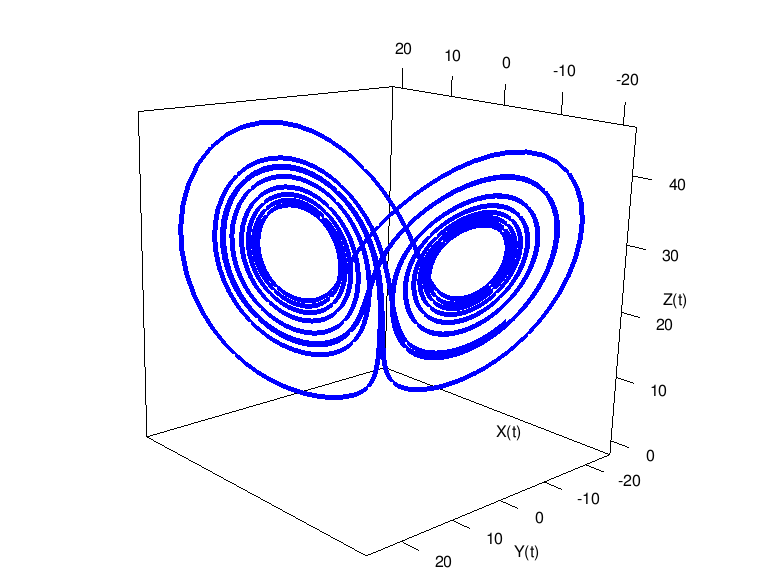
\includegraphics[scale=.25]{lorenzattractor}
%   \caption{$\sigma=10$, $\rho=28$ and $\beta=3/8$}
%        \end{figure}
%      \end{column}
%   \end{columns}
%  \end{frame}
% 
%  
%  
 
% 
% 
% %+++++++++++++++++++++++++++++++++++++++++++++++++++
% %%%%%%%%%%%%%%%
% %%ANIMATION in evince
% \begin{frame}
% \frametitle{Time-Delay Embedding Example}
% \vspace{-9mm}
% \begin{columns}[onlytextwidth]
%   \begin{column}{0.5\textwidth}
% \begin{figure}
% 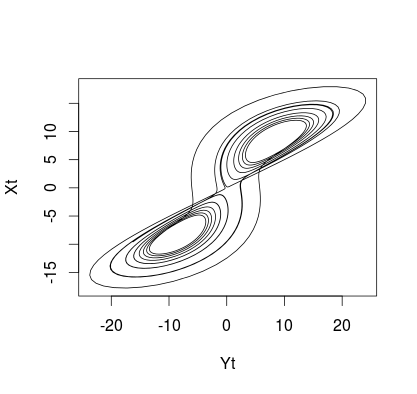
\includegraphics[scale=.3]{XY} 
% \caption{Original Manifold}
% \end{figure} 
% \end{column} 
% 
% \begin{column}{0.5\textwidth}
% 
% \begin{figure}
% \multiinclude[format=png,graphics={scale=0.25}]{images_frames_for_TAU/join} 
% % \includegraphics[scale=0.3]{images_frames_for_TAU/manifold_d3_t-10}
% \caption{Reconstructed Manifold}
% \end{figure}
% \end{column}
% \end{columns}
% \end{frame}
% 
% 
% 
% 






% 
% %+++++++++++++++++++++++++++++++++++++++++++++++++++
% \begin{frame}
% \frametitle{Quantifying Dexterity in Dance}
% \vspace{-0.6cm}
% \begin{figure}
% \includegraphics[scale=0.5]{beginner_salsa_steps_01} \\
% 
% \end{figure}  
% \end{frame}
% 
% 
% %+++++++++++++++++++++++++++++++++++++++++++++++++++
% \begin{frame}
% \frametitle{Phase Spaces for Dancing}
% \vspace{-0.6cm}
% \begin{figure}
% \includegraphics[scale=0.029]{results_v11} \\
% \end{figure}  
% \end{frame}

% %+++++++++++++++++++++++++++++++++++++++++++++++++++
% \begin{frame}
% \frametitle{$E1(d)$ and $E2(d)$ values}
% \vspace{-0.6cm}
% \begin{figure}
% \includegraphics[scale=0.07]{ev_gyr} \\
% 
% \end{figure}  
% \end{frame}
% 
% 
% %+++++++++++++++++++++++++++++++++++++++++++++++++++
% \begin{frame}
% \frametitle{$E1(d)$ and $E2(d)$ values}
% \vspace{-0.6cm}
% \begin{figure}
% \includegraphics[scale=0.07]{ev_mag} \\
% 
% \end{figure}  
% \end{frame}
% 



% 
% %+++++++++++++++++++++++++++++++++++++++++++++++++++
% \begin{frame}
% \frametitle{Percentages of variances}
% \vspace{-0.6cm}
% \begin{figure}
% \includegraphics[scale=0.15]{tables_v1} \\
% 
% \end{figure}  
% \end{frame}
% 
% 
% 
% 



% 
% 
% %+++++++++++++++++++++++++++++++++++++++++++++++++++
% \begin{frame}
% \frametitle{2-D reconstructed state spaces (RSS)}
% \vspace{-0.6cm}
% \begin{figure}
% \includegraphics[scale=0.09]{skills} \\
% 
% \end{figure}  
% \end{frame}
% 
% 
% 
% 
% 
% %+++++++++++++++++++++++++++++++++++++++++++++++++++
% \begin{frame}
% \frametitle{Different embedded parameters}
% \vspace{-0.6cm}
% \begin{figure}
% \includegraphics[scale=0.07]{takens} \\
% 
% \end{figure}  
% \end{frame}
% 





% 
% 
% 
% %+++++++++++++++++++++++++++++++++++++++++++++++++++
% \begin{frame}
% \frametitle{RSS for Feet Pattern 2 \\ Participan 0 (Woman)- IMU1 GYR Z }
% \vspace{-0.5cm}
% 
% \begin{figure}
% \centering 
% \includegraphics[scale=0.25]{woman0} \\
% \end{figure}
% 
% \end{frame}
% %---------------------------------------------------
% 
% %+++++++++++++++++++++++++++++++++++++++++++++++++++
% \begin{frame}
% \frametitle{RSS for Feet Pattern 2 \\ Participan 1 (Woman) - IMU1 GYR Z }
% \vspace{-0.5cm}
% 
% \begin{figure}
% \centering 
% \includegraphics[scale=0.25]{woman1} \\
% \end{figure}
% 
% \end{frame}
% %---------------------------------------------------
% 
% %+++++++++++++++++++++++++++++++++++++++++++++++++++
% \begin{frame}
% \frametitle{RSS for Feet Pattern 2 \\ Participan 2 (Man) - IMU1 GYR Z }
% \vspace{-0.5cm}
% 
% \begin{figure}
% \centering 
% \includegraphics[scale=0.25]{man0} \\
% \end{figure}
% 
% \end{frame}
% %---------------------------------------------------
% 
% %+++++++++++++++++++++++++++++++++++++++++++++++++++
% \begin{frame}
% \frametitle{RSS for Feet Pattern 2 \\ Participan 3 (Man) - IMU1 GYR Z }
% \vspace{-0.5cm}
% 
% \begin{figure}
% \centering 
% \includegraphics[scale=0.25]{man1} \\
% \end{figure}
% 
% \end{frame}
% %---------------------------------------------------
% 
% %+++++++++++++++++++++++++++++++++++++++++++++++++++
% \begin{frame}
% \frametitle{RSS for Pattern 2 \\ Participan 4 (Man) - IMU1 GYR Z }
% \vspace{-0.5cm}
% 

% 
% \end{frame}

% %---------------------------------------------------




\section{IMU Benchmark}

%+++++++++++++++++++++++++++++++++++++++++++++++++++
\begin{frame}
\frametitle{IMUs Benchmark -- Data that other use}
\vspace{-0.7cm}


\hspace*{-25mm} \includegraphics[scale=0.47]{imubenchmark.pdf} 

   

\end{frame}
%---------------------------------------------------






%+++++++++++++++++++++++++++++++++++++++++++++++++++
%+++++++++++++++++++++++++++++++++++++++++++++++++++
\section{Plan}

%+++++++++++++++++++++++++++++++++++++++++++++++++++
\begin{frame}
\frametitle{PhD Framework for February and March}
\vspace{-0.7cm}

% \begin{figure}
% \centering 
% \includegraphics[scale=0.26]{proposedapproach_v1} \\
% \end{figure}

\textbf{FEBRUARY}
    \begin{itemize}
    \item Create Artificial Structure Signals.
    \item Apply Statistical and Nonlinear methods to analise the variability of artificial signals.
    \item Pilot Data Collection Experiment Using Commertial and non-commertial IMUs.
    \end{itemize}
\textbf{MARCH}    
    \begin{itemize}
    \item Pilot classification experiment with SVM or a technique of deep learning \\ (collaboration with \textit{Dr. Mourad Oussalah})
    \item Submit the advances to the International Symposium on Wearable Computers (ISWC) 2016 (Deadline ist April 16, 2016)
    \end{itemize}    
    
%    Deep Convolutional and LSTM Recurrent Neural Networks for Multimodal Wearable Activity Recognition.
%Ordóñez FJ1, Roggen D2.

\end{frame}
%---------------------------------------------------




%  \section[allowframebreaks]{References}
 
 
% \begin{frame}{References}

%    \scriptsize
 \begin{frame}[fragile,allowframebreaks]{References}
  % In your presentation, remove `\nocite` here and
  % use `\cite` throughout the presentation.
  \nocite{*}
  
  \bibliographystyle{apalike}
  \bibliography{refslides}


%  \bibliography{D:/Gpai/Biblographies/library}
\end{frame}





%+++++++++++++++++++++++++++++++++++++++++++++++++++
\begin{frame}
\frametitle{}

\vspace{2cm}
\begin{center}
\LARGE{QUESTIONS?} 
\end{center}

\vspace{1cm}

\normalsize 
\textbf{Miguel Perez-Xochicale} \\

E-Mail: {\color{blue} \href{mailto:perez.xochicale@gmail.com}{perez.xochicale@gmail.com} } 

Homepage:
{\color{blue} \href{https://sites.google.com/site/perezxochicale/}{https://sites.google.com/site/perezxochicale/} }
\vspace{1cm}



\includegraphics[scale=.4]{CC4}
\tiny{ 
\textbf{My own pictures are release under CC BY-NC 4.0
{\color{blue} \href{http://creativecommons.org/licenses/by-nc/4.0/}{http://creativecommons.org/licenses/by-nc/4.0/} } \\
Give credits to: Miguel Perez-Xochicale
}
}

\end{frame}
%---------------------------------------------------

% 
% % Creates the cover page.
%  \frame{\titlepage}



\end{document}

